\chapter{Leeruitkomsten}
\label{ch:learning_outcomes}

%an introduction stating the learning outcome. (~50 words)
%a self-evaluation stating at what level of progression (see above), you believe you currently are for this learning
%outcome.
%a learning process description that supports your self-evaluation (why do you believe you have reached the
%above-mentioned level?), and the received feedback from the teachers and fellow students.
%Refrain from adding full pieces of work that can also be found in Canvas.
%Add a personal reflection on the received feedback: what do you think of it, and what did you do with it?
De leeruitkomsten die dit semester worden behandeld en ook moeten worden aangetoond zijn als volgt.

\begin{itemize}
	\item Ontwikkelen van bedrijfssoftware als teaminspanning
	\item Context Based Research
	\item Voorbereiding op levenslang leren
	\item Schaalbare architecturen
	\item Clouddiensten
	\item Veiligheid door ontwerp
	\item Gedistribueerde gegevens
\end{itemize}





\section{Ontwikkelen van bedrijfssoftware als teaminspanning}\label{sec:ontwikkelen-van-bedrijfssoftware-als-teaminspanning}

%Leeruitkomst 1 - Ontwikkeling en implementatie van bedrijfssoftware Je ontwikkelt en implementeert bedrijfssoftware
%zowel
%individueel als in teamverband met behulp van een geschikt bedrijfsontwikkelingsplatform en toepassingsraamwerk, volgens een professioneel softwareontwikkelingsproces.
%Je ontwikkelt dergelijke software in teamverband en houdt daarbij rekening met zowel functionele als niet-functionele eisen zoals gesteld door de stakeholders en de wetgeving.
%Verdere toelichting In dit semester wordt bedrijfssoftware gedefinieerd als grootschalige gedistribueerde software gericht op een organisatie en in staat om grote aantallen gelijktijdige gebruikers en gegevensoverdrachten te verwerken.
%Typisch is dat deze belasting niet gelijkmatig over de tijd is verdeeld.
%De ontwikkeling van bedrijfssoftware vindt plaats in teamverband volgens agile scrum.
%Het te ontwikkelen systeem voldoet zowel aan de functionele als aan de niet-functionele eisen die door de belanghebbenden worden gesteld.
%Het voldoen aan de functionele en niet-functionele eisen wordt aangetoond door (geautomatiseerde) tests.
%Daarnaast zal het systeem voldoen aan de General Data Protection Regulation (GDPR)


%Wat wil ik leren
	Dit semester wil ik leren om enterprise software op te leveren in teamverband, aan een echte klant.
	Hierbij bespreken we samen met de klant zijn wensen en functionaliteiten.
	Voor deze samenwerking ga ik de Agile Scrum methodiek gebruiken.
	Daarnaast moet het systeem dat door ons als groep wordt ontwikkeld voldoen aan de GDPR-wetgeving.


%Wat moet ik doen om dit te kunnen bereiken?
	Dit leerdoel ga ik bereiken door een strakke planning en goede communicatie met het team en klant.
	Ook zullen we samen technische aspecten bespreken en doelgericht onderzoek uitvoeren om zo tot oplossingen te komen
	voor onze problemen.


%Welke middelen heb ik hiervoor nodig?
	Hierbij is het van belang een gemotiveerd team te hebben met leergierigen individuen en een klant die pro-actief
	meedenkt over wat hij wil in het eindproduct.
	Communicatie is hierbij belangrijk met het team, maar ook met de externe partijen.

	Tijdens ons groepsproject is er communicatie met verschillende teams en contact personen.
	Zo is er een groep bezig aan de front-end en is er een afstudeer student bezig met de technische kant van de front-end.


%Hoe ga ik success meetbaar maken?
	Ik ga dit leerdoel meetbaar maken door middel van een evaluatie op het einde van elke sprint.
	Hierbij noteer ik mijn sterke en zwakke punten die worden aangekaart door mijn team zodat ik deze in de toekomst kan verbeteren.
	Ook is het project en de deelproducten die wij als groep opleveren een goede indicatie van mijn bekwaamheid tot deze leeruitkomst.

	\newpage
	\bigskip



	\subsection{Ontwikkel process}
%Evaluatie hoe heb ik het bereikt?

%SPRINT 0 =============================================
	\subsubsection{Sprint 0}
	\paragraph{Evaluatie: 12-03-2021}
	Dit is de ontdekkingsfase; wat is het project, welke technieken komen erbij kijken
	en welke technieken kunnen we het beste toepassen voor ons project.
	Hoe gaan we als groep een succesvol project opleveren voor onze klant; wat zijn functionele- en non functionele eisen/wensen.
	Hierover hebben we samen met de klant gesproken in verschillende "online" bijeenkomsten.
	De uitkomsten hiervan zijn vastgelegd in de deel documenten. Deze zijn terug te vinden in het canvas dashboard.


	Hieronder is een opsomming van de uitkomsten die de professionaliteit van de sprint evalueren.
	Hierbij heb ik persoonlijk aan mijn teamleden gevraagd waar voor mij verbetering ligt bij deze sprint.
%Sterke punten
	\subparagraph{Sterke punten:}
	\begin{itemize}
		\setlength{\itemsep}{0pt}%
		\setlength{\parskip}{0pt}%
		\item Denkt diep na over een topic en brengt een goed technisch beeld over naar teamgenoten
		\item Levert een goede bijdrage aan het ontwikkelen
	\end{itemize}

%Verbeter punten
	\subparagraph{Verbeter punten:}
	\begin{itemize}
		\setlength{\itemsep}{0pt}%
		\setlength{\parskip}{0pt}%
		\item Nog n.v.t.
	\end{itemize}


%Evaluatie hoe heb ik het bereikt?

%SPRINT 1 =============================================
	\subsubsection{Sprint 1}
	\paragraph{Evaluatie: 01-04-2021}
	Dit was onze eerste sprint. Tijdens deze sprint hebben we de opdracht vastgesteld en een ontwerp gemaakt van ons project.
	Bij het maken van het ontwerp was het belangrijk ervoor te zorgen dat de app een modulaire opbouw krijgt, wat er voor zorgt dat het goed overdraagbaar is.
	Om deze modulariteit te behalen hebben we gekozen voor een microservice architectuur.
	Het is belangrijk dat het project overdraagbaar is, omdat dit project in de toekomst zal worden door ontwikkeld door externe project groepen.
	Ook is het van belang dat het ontwerp aan de "GDPR" regelgeving voldoet.
	De GDPR-regelgeving beschermt de gebruiker en zijn gegevens in ons systeem.
	Ook hebben we tijdens deze sprint verschillende prototypes gemaakt waarvan de klant zeer onder de indruk was.
	In deze prototypes hebben we nieuwe technische methodes uitwerkt en getest, die we laten willen gaan toepassen in het definitieve project.
	Deze ontwerpen en prototypes zijn ook besproken met vak experts / docenten.
	Dit stelt de kwaliteit vast van onze deelproducten en zo kunnen we vroegtijdig de nodige wijzigingen aanbrengen.
	Ook is deze documentatie belangrijk voor de overdraagbaarheid aan een toekomstig team die aan dit project verder
	zullen gaan werken.


	Hieronder is een opsomming te vinden van de eindbespreking van sprint 1.
	Hierbij hebben we net zoals voorgaande sprint de tips en tops besproken en waar voor mij verbeteringen liggen in de
	sprints die nog komen.
%Sterke punten
	\subparagraph{Sterke punten:}
	\begin{itemize}
		\setlength{\itemsep}{0pt}%
		\setlength{\parskip}{0pt}%
		\item Initiatief nemend.
		\item Gemotiveerd en leergierig.
		\item Brede technische kennis.
		\item Je zoekt dingen tot het bot uit.
		\item Algemene samenwerking; je helpt waarnodig mee en helpt anderen goed.
	\end{itemize}

%Verbeter punten
	\subparagraph{Verbeter punten:}
	\begin{itemize}
		\setlength{\itemsep}{0pt}%
		\setlength{\parskip}{0pt}%
		\item Te lang zichzelf vast kunnen klampen aan een ding.
		Perfectie is een streven maar het moet niet tegen werken.
		\item Je kan meer initiatief tonen om aan nieuwe zaken te beginnen wanneer je huidige af zijn.
	\end{itemize}

	\bigskip

%SPRINT 2 =============================================
	\subsubsection{Sprint 2}
	\paragraph{Evaluatie: 23-04-2021}
	Dit was onze eerste echte print oplevering waar we ook echt code gingen opleveren.
	Hierbij werken we volgens de agile scrum methodiek en hebben we elke 2 weken een sprint oplevering.
	Deze sprint oplevering presenteren we ons werk voor de verschillende teams, de project eigenaar Wouter en
	natuurlijk bespreken we naderhand hoe de oplevering is gegaan met onze docenten.
	Door de positieve feedback en de goede samenwerking en teaminspanning bij het project kan ik mijzelf
	beoordelen met een "proficient".
	Natuurlijk zijn we nog niet op het einde van het semester daarom zie ik deze proficient onder voorbehoud.
	In de aankomende sprint ga ik deze beoordeling definitief maken.





%Eigen beoordeling
\subsection{Eind beoordeling / reflectie}
%Wij als groep hebben een mooi degelijk product opgeleverd.
%In dit project zijn alle wensen verwerkt die door de klant werden opgedragen.
%Ook hebben we in dit project alle technieken die voor dit semester van toepassing waren verwerkt.
%Dit project kan in de toekomst verder worden doorontwikkeld door andere project groepen.
%
%\bigskip
%Door de behaalde resulaten difinieer ik mijn bekwaamheid tot dit leerdoel als:\\
%\par\vspace{10pt}\textbf{\uppercase{"Proficient"}}\\
	Binnen ons team is er een ontzettend goede communicatie. Afspraken waren daarom ook duidelijk binnen het gehele team.
	Ook ondersteunde we elkaar waar nodig, sommigen meer dan anderen maar over het algemeen ben ik zeer tevreden.

\newpage

%! Author = rikpe
%! Date = 24/04/2021

\section{Context Based Research}\label{sec:context-based-research}

%Leeruitkomst 2 - Contextgericht onderzoek Je onderbouwt je keuzes voor processen en technieken aan de hand van een
%algemeen geaccepteerde onderzoeksmethode en rekening houdend met je eigen ethische waarden.
%Verdere toelichting Je onderbouwt je keuzes voor processen en technieken aan de hand van contextgebaseerd onderzoek.
%Je maakt gebruik van bekende en algemeen geaccepteerde onderzoeksmethoden of -modellen, zoals het DOT Framework en
%ICT Research Methods.
%Je communiceert je onderzoeksaanpak, plan, resultaten en conclusie zowel mondeling als schriftelijk.

%Wat wil ik leren
Dit semester wil ik leren om doelgericht onderzoek te doen waarvan de uitkomsten kunnen bijdragen aan het ontwikkelen van technische en complexe software oplossingen.
Onderzoek is nodig om kennis op te doen bij een bepaald onderwerp en om deze zo beter te kunnen begrijpen.
Vanuit daar kun je je kennis stapsgewijs (onderzoek voor onderzoek) opbouwen om zo tot een gepaste oplossing te
komen voor een probleem.


%Wat moet ik doen om dit te kunnen bereiken? / %Welke middelen heb ik hiervoor nodig?
Door de onderzoeksmethodieken te gebruiken die in het DOT-framework staan omschreven kan ik doelgericht onderzoek
doen.
Voor het onderzoek ga ik verschillende methodieken combineren om zo tot een oplossing te komen op mijn probleem.


%Hoe ga ik success meetbaar maken?
Dit leerdoel ga ik meetbaar maken door onderzoeksdocumenten op te leveren die door zowel mij als door een ander als
nuttig worden beschouwd en daarmee ook een bijdrage kunnen leveren aan een oplossing van een complex probleem.
Ik definieer mijn kwaliteit op de feedback die ik heb ontvangen van vak bekwame experts "docenten".

%Wat heb ik gedaan om dit aan te tonen?
Bij zowel het groepsproject als het individueel project heb ik verschillende casestudies gemaakt die voor een klant
kunnen helpen bij het maken van een keuze om zo een probleem op te lossen.

\bigskip
\subsection{Ontwikkel process}
%evaluatie / %Beoordeling
\subsubsection{Case Studies}
\paragraph{Evaluatie: 24-04-2021}
Tijdens het groepsproject hebben we zes verschillende case studies moeten uitwerken.
Deze case studies gaven een complex probleem weer waar een oplossing bij gevonden moest worden.
De problemen deden zich voor op verschillende aspecten binnen het ontwikkelen van software.
De case studies zijn uitgewerkt door middel van het toepassen van verschillende methodieken uit het DOT-framework.
De casestudies die tijdens het proftaak groepje zijn behandeld, zijn goed afgerond en de feedback van de leraren is
verwerkt.
Daarom beschouw ik mijn huidige oriëntatie als "georiënteerd".
Deze case studies zijn terug te vinden in het canvas bij he opdrachtenoverzicht van project groep 3.
Bij de verschillende case studies hebben we taken verdeeld. Mijn bijdrage aan de case studies zijn als volgt:

\begin{itemize}
	\setlength{\itemsep}{0pt}%
	\setlength{\parskip}{0pt}%
	\item Gebrainstormd over de case studie; wat houdt deze in en wat vragen ze van ons
	\item Onderzoeksvragen opgesteld gebaseerd op de brainstorm sessie
	\item Onderbouwde feedback gegeven op elkaars uitwerking op een vraag en waar nodig ondersteund.
	\item Onderzoeksvragen en deelvragen uitgewerkt.

\end{itemize}

Gebaseerd op de feedback van onze docenten ligt onze kwaliteit hoog.
Alle feedback die we ontvangen wordt genotuleerd en wordt in de volgende case studie meegenomen.

\subsubsection{Onderzoek}
\paragraph{Evaluatie: 05-04-2021}
Voor het individuele project heb ik ook context based research toegepast voor het "cache van data binnen mijn project".
Ook tijdens dit onderzoek is het dot onderzoeks framework toegepast.
Uit het dot framework heb ik de volgende methodes uitgekozen:

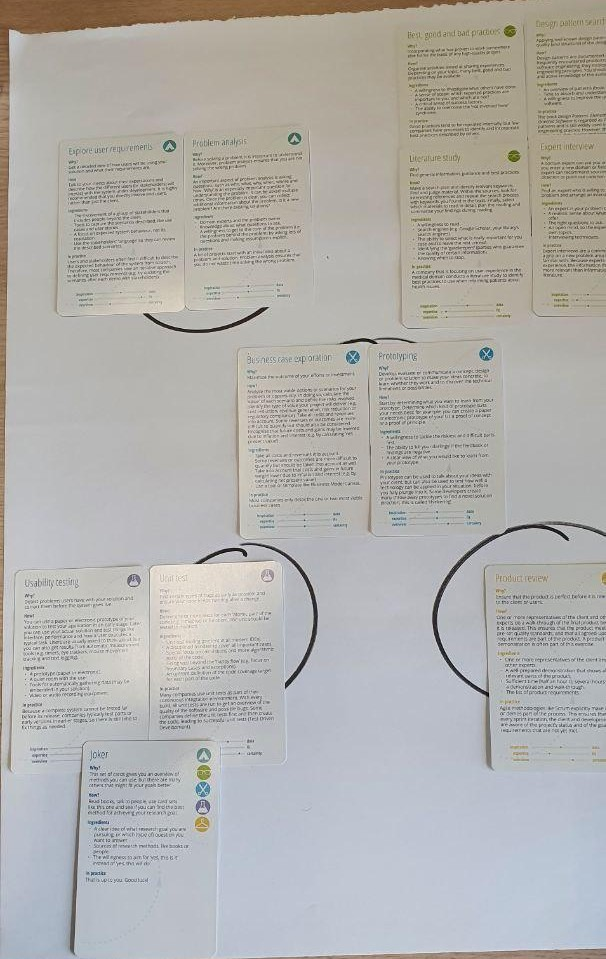
\includegraphics[width=\textwidth,height=\textheight,keepaspectratio]{Context_Based_Research_Defined_Research_Methodes.jpg}\label{fig:research_methodes}

Deze methodes zijn besproken met Tom Langhorst docent gespecialiseerd het contextueel onderzoeken.

De onderzoeks vraag luid als volgt: "Hoe wordt caching toegepast op enterprise software niveau voor specifieke doeleinde binnen het java framework springboot?"

Tijdens het onderzoek zijn de toepassingen van caching mijzelf zeer duidelijk geworden.
Bij het onderzoek hebben we ook enkelen prototypes gemaakt de de snelheid en de toepassing van caching goed laat zien.
Na het prototype hebben we aan een vak expert om feedback gevraagd tijdens dit feedback moment hebben we het over verschillende topics gehad bij komen kijken bij het cachen van data.


\subsection{Eind beoordeling / reflectie}
Ik ontzetten veel geleerd over de contextueel onderzoek doen naar een topic en heb geleerd hoe ik een onderzoeksvraag moet samenstellen.
Gebaseerd op de verschillende case studies en groeps onderzoeken en het individueel onderzoek beschouw ik mijn huidige bekwaamheid tot dit leerdoel op:\\
\par\vspace{10pt}\textbf{\uppercase{"Proficient"}}\\


\newpage

%! Author = rikpe
%! Date = 24/04/2021

\section{Voorbereiding op levenslang leren}\label{sec:voorbereiding-op-levenslang-leren}
%Leer uitkomst 3 - Voorbereiding op levenslang leren Je signaleert opkomende trends in software engineering,
%onderzoekt ze en past ze waar nodig toe in je projecten.
%Ook ben je je bewust van mogelijke carrièrepaden en je verwerft de vereiste vaardigheden om voorbereid te zijn op je
%toekomstige carrière.
%Verdere toelichting Niet alle opkomende trends komen aan bod in de andere eindtermen.
%Opkomende trends zijn ook Domain-Driven Design, Blockchain, Programmeerparadigma's, Machine Learning, en Quantum
%Computing.
%De genoemde onderwerpen komen in het studiemateriaal aan bod.
%Je kiest één van deze onderwerpen in overleg met je tutorgroep en docenten.
%Carrièrepaden zullen per student verschillen.
%Software engineers kunnen bijvoorbeeld doorgroeien naar software architect of teamleider.
%Studenten die zich specialiseren in bijvoorbeeld cybersecurity, toegepaste data science of game design kunnen een
%ander carri.èrepad hebben dan studenten die zich specialiseren in software engineering.
%Je moet je bewust zijn van je eigen carrièrepad en de vaardigheden die voor die rol vereist zijn.
%Je moet bereid zijn om de volgende stap te zetten om je vaardigheden te ontwikkelen, wat een minor of een
%afstudeerproject kan betekenen.

%Wat wil ik leren
Voor mijn studie worden veel nieuwe technieken aangedragen door school, maar hoe ga ik er in de toekomst zelf voor
zorgen dat ik up-to-date blijf met de laatste trends die zich in de ICT-wereld ontwikkelen.
Hiervoor is het daarom belangrijk nu al na te denken over hoe ik dit ga aanpakken.
Daarom wil ik dit semester leren om mijzelf voor te bereiden om levenslang te leren.

%Wat moet ik doen om dit te kunnen bereiken? / %Welke middelen heb ik hiervoor nodig?
Om dit te kunnen bereiken moet ik mijzelf blijven motiveren om door te leren na mijn studie.
Dit kan zowel door cursussen te volgen als door zelfstudie met doelgericht onderzoek naar nieuwe
ontwikkelingen binnen de ICT-wereld.
Door up-to-date te blijven van de nieuwste ontwikkelingen blijf ik als software engineer goed op de markt liggen.

%Hoe ga ik success meetbaar maken?
Dit leerdoel is meetbaar te maken door het toepassen van deze nieuwe technieken binnen mijn toekomstige projecten.

\subsection{Toegepaste technieken}\label{subsec:toegepaste-technieken}
Hieronder bespreek ik hoe ik verschillende technieken heb onderzocht en toegepast.
Deze technieken waren voor mij nog van onbekend terrein.
De definitie van life nog learning is het analyseren en het toepassen van nieuwe 'Trends' technieken.
Deze trends laat ik hieronder zien.
%Wat heb ik gedaan om dit aan te tonen?

Hoe ga ik nieuwe trends ontdekken?
Dit ga ik doen door actief online in te zoeken naar methodieken die voor mij een bepaald probleem oplossen of zelf
vermakelijken.
Wanneer ik ontdek dat ik bij een techniek mijzelf repeteer en onnodig een complexe oplossing hierbij ga zoeken.
Ga ik online zoeken hoe andere mensen tot een oplossing zijn gekomen als zei mij vervolgens informeren dat hier een
nieuwe oplossings- trend in is ontwikkeld ga ik hier zelf mee experimenteren.
Ook op youtube volg ik veel vak experts die nieuwe technieken analyseren en hier een eigen visie aan geven.
Wanneer deze experts een goede onderbouwen waarom het toepassen van deze trend een prositieve invloed zal hebben op
toekomstige projecten zal ik hier zelf natuurlijk ook mee gaan experimenteren.
Daarom geeft youtube voor mij een zeer goede bijdragen aan het voordragen van nieuwe 'trends' en technieken.
Wanneer ik met een probleem zit ga ik persoonlijk op stackoverflow zoeken naar oplossingen van andere mensen.
Hierbij komst het ook voor dat deze personen mij introduceren aan een nieuwe techniek en de toepassing hiervan.
Zelf houd ik van een “gedecentraliseerde” informatie voorziening.
Hiermee bedoel ik dat een bedrijf mij niet een nieuwe techniek moet aandragen voor hun eigen gewin.
Ik moet zelf hier de toegevoegde waarden van inzien en dit doe ik door verschillende bronnen te raadplegen.


\subsubsection{Microservices}
\paragraph{Eerste evaluatie - 16-03-2021}
Voor mijn individueel project ben ik bezig aan een distributie app.
Context over dit project is te lezen in de inleiding
Deze distributie app ga ik ontwikkelen met een modulaire architectuur die bestaat uit microservices.
Helaas wist ik op het begin nog vrij weinig wat microservices inhielden en voor welke toepassingen ze werden gebruikt.
Na onderzoek en verschillende prototypes heb ik mijzelf wegwijs gemaakt in de toepassing hiervan.

Voor mijn individueel project ben ik begonnen met een ontwerp en verschillende workflows die deze app zou moeten gaan automatiseren.
Vervolgens ben ik begonnen met het ontwikkelen prototypes specifiek op het project in deze prototypes heb ik ook de technieken uitgewerkt die ik van plan was te gaan te gebruiken
Vervolgens ben ik deze prototypes gaan bespreken met Software docente Merel.
Hierbij heb ik de verschillende technieken laten zien die ik van plan was te gaan gebruiken bij deze technieken kun je bijvoorbeeld denken aan HATEOAS HAL en springboot cloud gateway.
Dit zijn allemaal technieken die zorgen voor modulariteit binnen mijn microservices.
De terugkoppeling die ik hierbij heb ontvangen was positief en we hebben tijdens dit terugkoppeling moment ook over complexe ideologieën gesproken, zoals de generieke response content types van mijn rest api.
Na dit gesprek heeft merel geconstateerd dat mijn bekwaamheid tot verschillende leerdoelen op "beginning" mag worden gezet.


\subsubsection{Deployment en schalen}
\paragraph{Eerste evaluatie - 02-03-2021}
De eerste weken heb ik onderzoek gedaan hoe Docker werkt en hoe ik een image kan maken van een project.
Vervolgens heb ik een compose file gemaakt die het mogelijk maakt verschillende images tegelijkertijd te starten.

Met deze compose files heb ik vervolgens een github actions (CI/CD) workflow aangemaakt die de verschillende testen automatiseerde.
Deze workflow in te zien in de project repositorie op github.

De volgende stap is het deployen van deze image naar een cloud omgeving om zo de app live te zetten.

\subsubsection{Protocollen}\label{subsec:protocollen}
\paragraph{Eerste evaluatie - 02-03-2021}
De eerst weken heb ik onderzoek gedaan naar de verschillende protocollen die worden gebruikt voor het streamen van data.
Dit was van belang voor het groepsproject waarbij een online video platform moet worden ontwikkeld.
Welke protocollen passen bijvoorbeeld het beste bij het huidige groepsproject.
UTP of TCP / RTMP of webrtc of zelf een ander protocol.
Hierbij heb ik gekeken hoe bekende streaming diensten tot een oplossing zijn gekomen en waarom dat ze voor een
bepaald protocol hebben gekozen.
Hierbij ben ik tot de conclusie gekomen dat voor onze toepassing heb beste kan worden gewerkt met webrtc.
Webrct is een opvolger van het verouderde maar nog steeds veel gebruikte RTMP-protocol.

\subsubsection{Gateway}\label{subsec:gateway}
\paragraph{Eerste evaluatie - 20-04-2021}
Omdat mijn applicatie met een microservice architectuur werkt en omdat het van belang is dat de frontend goed kan communiceren met deze back-end.
Het ik er voor gekozen om een gateway te implementeren.
Een gateway is een soort van service balie van een applicatie die je naar de juiste plek verwijst.
Elke microservice binnen mijn app heeft zijn eigen poort wanneer deze vervolgens gaat schalen kunnen dit er nog meer worden.
Als oplossing hiervoor heb ik gekozen om Zuul gateway in combinatie met Eureka discovery te implementeren.
Deze dependencies zijn beide ontwikkeld door Netflix.
Eureka kan automatisch zien wanneer een applicatie zich 'aanmeld' wanneer er dus een request naar de Zuul gateway
wordt gestuurd kan zuul aan eureka vragen wat het juiste doorverwijs adres is.

Hieronder een afbeelding van de microservices die zich aan hebben gemeld bij eureka.
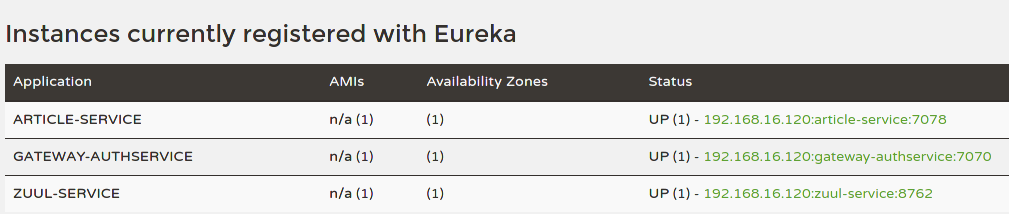
\includegraphics[width=\textwidth]{Eureka_Discovery.png}\label{fig:eureka_discovery}


\subsection{Eind beoordeling / reflectie}
Door het uitwerken van verschillende trends binnen zowel het individueel als het groepsproject oriënteer ik mijzelf
als "proficient" de bewijs last van het toepassen van deze technieken zijn zowel hierboven omschreven en terug te
vinden in de implementatie binnen de projecten.

\newpage

%! Author = rikpe
%! Date = 24/04/2021

\section{Schaalbare architecturen}\label{sec:schaalbare-architecturen}
%Leer uitkomst 4 - Schaalbare architecturen Je ontwikkelt bedrijfssoftware op basis van een gekozen gedistribueerde
%architectuur die duidelijk schaalbaarheid ondersteunt voor hoog volume communicatie en event handling, en
%onafhankelijk life cycle management mogelijk maakt.
%Verdere toelichting Tegenwoordig zijn schaalbare architecturen vaak gebaseerd op microservices.
%Microservices maken fijnkorrelige services in een gedistribueerd systeem mogelijk, waarbij elke service zijn eigen
%levenscyclus heeft.
%Je definieert interfaces tussen microservices met behulp van event storming, wat een workshop-gebaseerde methode is
%om alle relevante gebeurtenissen te ontdekken die binnen het domein van het bedrijfssysteem plaatsvinden.
%Je implementeert samenwerking tussen services met behulp van event sourcing technieken.
%Je documenteert je architectuurontwerp met diagrammen volgens een ontwerpproces.


%Wat wil ik leren
Ik wil leren hoe ik enterprise software maak die schaalbaar en gedistribueerd is.
Binnen de enterprise software moeten de microservices onafhankelijk van elkaar opereren.
Microservices zijn onafhankelijke programma's die met elkaar kunnen communiceren door middel van protocollen.
Dit is mogelijk door een goed technische ontwerp van het op te leveren product.
Dit ontwerp wordt gedocumenteerd in verschillende technische documenten zoals het Software Architecture Document (SAD).

%Wat moet ik doen om dit te kunnen bereiken?
Hierbij is het van belang dat ik de nodige kennis op doe over microservices.
Daarnaast zal ik onderzoek moeten doen naar hoe deze protocollen onderling werken en hoe ik deze moet toepassen.

%Welke middelen heb ik hiervoor nodig?
Hierbij is het ook van belang om goede tooling toe te passen zoals UML of C4 voor een goed technische ontwerp.
Bij het ontwikkelen is het ook belangrijk om een goede en intelligente IDE te gebruiken, zodat ik efficient te werk
kan gaan.

%Hoe ga ik success meetbaar maken?
Ik ga dit leerdoel meetbaar maken door een goed project op te leveren, zowel voor het individueel project als het
groeps project.
Hierbij is het belangrijk dat ik stevige argumenten heb om mijn keuzes te onderbouwen die ik heb gemaakt tijdens
het ontwikkel process.
Het project moet natuurlijk schaalbaar zijn dit ga ik aantonen door een microservice architectuur toe te passen.

Dit leerdoel sluit ook goed aan bij het leerdoel "Voorbereiding op levenslang leren". In dit hoofdstuk omschrijf ik
hoe ik microservices heb toegepast voor mijn individueel project.
Graag wil ik u, de lezer, dan ook verwijzen om meer te lezen over microservices in dat hoofdstuk.












\newpage

%! Author = rikpe
%! Date = 24/04/2021

\section{Ontwikkeling en uitvoering (DevOps)}\label{sec:ontwikkeling-en-uitvoering-(devops)}
%Leer uitkomst 5 - Development and Operations (DevOps) Je zet een omgeving en teamprocessen op die een volledig
%geautomatiseerde softwarelevenscyclus ondersteunen, terwijl je een hoge kwaliteit, hoge beschikbaarheid, snelle
%levering en korte releasetijden garandeert.
%Verdere verduidelijking Wijzigingen in de software worden ingevoerd in een goed gedefinieerd proces volgens change
%management en release procedures.
%U ontwikkelt bedrijfssoftware met behulp van CI/CD-pijplijnen.
%I/CD staat voor continuous integration en continuous delivery en/of continuous deployment.
%De CI/CD-pijplijn voert geautomatiseerde tests uit, waaronder unit tests, component tests, integratietests en
%gebruikersacceptatietests.
%Daarnaast wordt een rapport over code coverage en statische code kwaliteit gegenereerd.
%De CI/CD pipeline, testomgeving en deployment worden gecontaineriseerd.
%De implementatie van (micro)services zal worden opgeschaald wanneer nodig met behulp van container orchestration.


%Wat wil ik leren / %Wat moet ik doen om dit te kunnen bereiken? / %Welke middelen heb ik hiervoor nodig?
Voor dit leerdoel wil ik leren hoe ik een automatische test pipeline (CI/CD) opzet door middel van Github actions.
Hierbij wordt een automatische test flow opgezet die valideert of een build is geslaagd.
Wanneer deze build en de daarbij horende testen succesvol zijn uitgevoerd, wordt de image naar een production environment gestuurd waarna
de software vervolgens live wordt gezet en gebruikt kan worden door de klant.
Dit gebeurt door middel van een Kubernetes cluster.
Ook ga ik tooling gebruiken voor het bijhouden van de te ontwikkelen functionaliteiten.
Hierbij wordt in het groepsproject Devops gebruikt en voor mijn individueel project ga ik hier het Github issue-board voor gebruiken.

%Hoe ga ik success meetbaar maken?
Dit leerdoel is meetbaar te maken door de leraar proactief te informeren over hoe het ontwikkelproces zich vordert.
Ook ga ik mijn Github actions CI/CD pipeline laten zien waar de code wordt gecontroleerd op geslaagde testen en kwaliteit.
De kwaliteit van de code word getest met SonarCloud.


\subsection{Ontwikkel process}
\subsubsection{Github actions}
\paragraph{Evaluatie: 05-04-2021}
Voor het toepassen van de CI/CD pipeline verwacht ik niet enorm veel werk.
Dit is mede omdat ik in semester drie maar ook in vier hier al mee heb gewerkt en dit al eerder heb geïmplementeerd.
Daarom zie ik tijdens dit semester meer mogelijkheden voor verbetering van dit proces.
Voor mijn CI/CD module heb ik gekozen voor het toepassen van Github actions.
Mijn pipeline controleert op zowel geslaagde testen als op de code kwaliteit.
Elke microservice binnen mijn applicatie heeft zijn eigen pipeline met checks.
Hieronder is de uitwerking van een van deze pipelines voor de microservice "Article".
Hierbij is te zien dat deze pipeline verschillende checks heeft waar hij doorheen loopt.\\

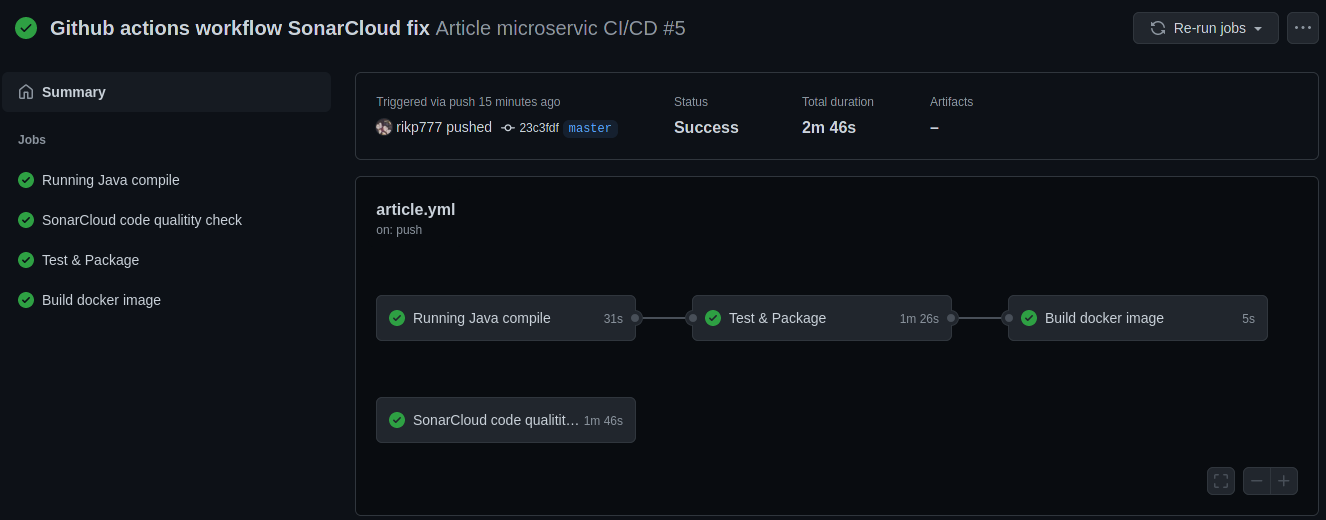
\includegraphics[width=\textwidth]{Article_Service_CI_CD_Pipeline.png}\label{fig:figure}


Via SonarCloud wordt de code gecontroleerd op kwaliteit en wordt aangekaart welke verbeteringen er kunnen plaatsvinden.\\

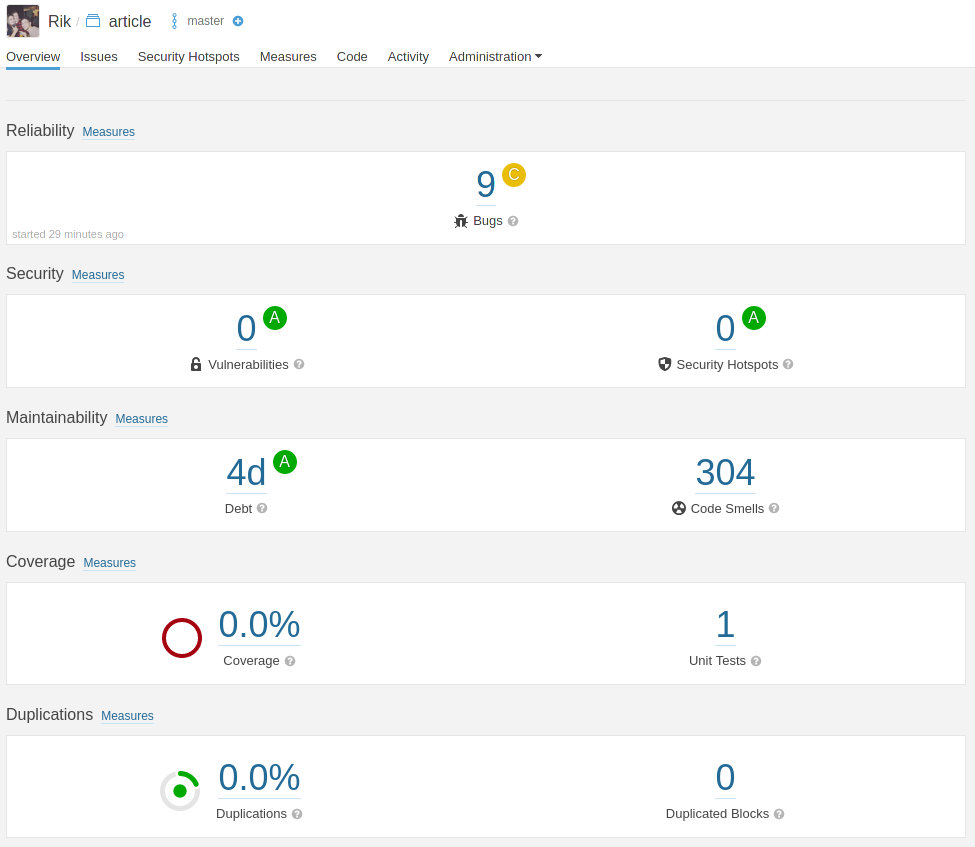
\includegraphics[width=\textwidth]{Article_Code_Quality_SonarCloud.png}\label{fig:figure2}


Omdat ik een gehele CI/CD pipeline heb geïmplementeerd voor mijn individueel project en mede door de uitwerking hierboven oriënteer ik mijzelf als:
\par\vspace{10pt}\textbf{\uppercase{"Proficient"}}.\\

Ik zou de beoordeling kunnen verbeteren naar een 'outstanding' door middel van het implementeren van een kubernetes cluster.

\subsection{Eind beoordeling / reflectie}
%Omdat ik een gehele CI/CD pipeline heb geimplementeeerd voor mijn individuele project door de uitwerking hierboven oriënteer ik mijzelf als proficient:
%\par\vspace{10pt}\textbf{\uppercase{"Proficient"}}\\




















\newpage
\section{Clouddiensten}\label{sec:clouddiensten}
%Leer uitkomst 6 - Cloud Services Je integreert cloud services en serverless computing technieken die je enterprise
%applicatie ondersteunen en er goed bij passen.
%Je onderzoekt de kosten en hoeveelheid resources die nodig zijn voor je applicatie.
%Je keuzes voor cloudprovider en ondersteunde tooling zijn gebaseerd op de belangen van stakeholders.
%Verdere toelichting Mogelijke clouddiensten zijn schaalbare databases, authenticatie, logging, monitoring, virtuele
%machines, en containerisatie.
%Het is ook mogelijk om een (micro)service in te zetten door alleen broncode aan te leveren, dit wordt serverless
%computing of function as a service (FAAS) genoemd.
%Je kent de voor- en nadelen van FAAS ten opzichte van containerisatie en je bent je bewust van de kosten die gepaard
%gaan met clouddiensten.

Nog niet van toepassing








\newpage
\section{Veiligheid door ontwerp}\label{sec:veiligheid-door-ontwerp}
%Leer uitkomst 7 - Security by Design Je integreert authenticatie en autorisatie, en beperkt mogelijke
%beveiligingsinbreuken tijdens het ontwerp en de implementatie van bedrijfssoftware.
%Verdere toelichting Je onderzoekt mogelijke beveiligingsinbreuken door misbruikgevallen te definiëren en je houdt
%rekening met deze gevallen tijdens het ontwerp en de implementatie.
%Je implementeert authenticatie en autorisatie met behulp van tooling en libraries die door enterprise software
%frameworks worden geleverd.
%Je bent op de hoogte van de meest kritische beveiligingsrisico's en je zorgt ervoor dat deze risico's voor jouw
%applicatie worden geminimaliseerd door de OWASP top 10 beveiligingsrisico's van webapplicaties aan te pakken.

%Wat wil ik leren
Voor het ontwikkelen van software is het van groot belang dat je software ook veilig is en voldoet aan de norm die
wordt gesteld.

%Wat moet ik doen om dit te kunnen bereiken?
Ik ga de OWASP top 10 beveiligingsrisico's goed door te nemen en de zaken die ik in het vorige semester heb
gedocumenteerd en onderzoek toepassen in zowel het groeps als het individueel project.

%Welke middelen heb ik hiervoor nodig? /%Hoe ga ik success meetbaar maken?
Door middel van het implementeren van HATEOAS Hal, OAuth2 en Spring Security ga ik aantonen dat ik over deze
technieken beschik en dat ik mijn software op deze manier veilig kan maken.
Ook ga ik proberen mijn software te kraken met de kennis die ik heb opgedaan uit de twee security specialisatie
semesters.


\subsection{Ontwikkel process}
\subsubsection{JWT Tokens}
Een JSON Web Token (JWT) is een op zichzelf staande manier definieert voor het veilig verzenden van informatie tussen partijen als een JSON-object.
Deze informatie kan worden geverifieerd en vertrouwd omdat ze digitaal ondertekend is.
JWT's kunnen worden ondertekend met een geheim of een openbaar/particulier sleutelpaar.
\paragraph{Evaluatie: 20-04-2021}
Voor mijn authenticatie en authenticatie gebruik ik JWT tokens in de vorm van een bearer.
Bearer authenticatie (ook wel token authenticatie genoemd) is een HTTP-authenticatieschema dat gebruik maakt van beveiligingstokens die bearer tokens worden genoemd.
De naam "Bearer authenticatie" kan worden opgevat als "geef toegang aan de drager van dit token".
Het bearer token is een cryptische string, meestal gegenereerd door de server in antwoord op een login verzoek.
De client moet dit token meesturen in de Authorization header wanneer hij verzoeken doet aan beschermde bronnen:
In mijn applicatie gebruik ik een token voor het authorizeren van interacties met mijn rest api.
Elke microservice binnen mijn applicatie heeft een Token nodig wanneer er een request wordt gestuurd.
Voor mijn eerste implementatie heb ik ervoor gezorg dat het artikel service kan worden geautoriseerd.


\subsubsection{HATEOAS HAL}
HATEOAS (Hypermedia as the Engine of Application State) is een beperking van de REST architectuur die de RESTful-stijlarchitectuur uniek houdt ten opzichte van de meeste andere toepassingsarchitecturen.
De term "hypermedia" verwijst naar alle inhoud die links bevat naar andere vormen van media, zoals afbeeldingen, films en tekst.
Dit houdt dus in dat een api interactief kan worden gemaakt en dat het makkelijk is om naar relational data te verwijzen.
\paragraph{Evaluatie: 20-04-2021}
Omdat ik gebruik maar van microservices is het handig als een frontend makkelijk naar relationele data kan verwijzen.
Dit doe ik door middel van HATEOAS met een gestandaardiseerde vorm in HAL formaat





\newpage
\section{Gedistribueerde gegevens}\label{sec:gedistribueerde-gegevens}
%Leer uitkomst 8 - Gedistribueerde data Je bent je bewust van data-eisen en je ontwikkelt bedrijfssystemen die
%gebruik maken van gedistribueerde data tooling en best practices.
%Je hebt een kritische houding ten opzichte van mogelijke privacy en ethische kwesties.
%Verdere toelichting Je definieert data-eisen, gebaseerd op de context van de data, de architectuur van het systeem,
%de infrastructuur, en (niet-)functionele eisen.
%Je bent op de hoogte van de beschikbaarheid van verschillende soorten gedistribueerde data-tooling en hun
%onderscheidende kenmerken en verschillende toepassingsgebieden.
%Je integreert gedistribueerde data tooling en best practices in de architectuur van je systeem en onderbouwt waarom
%deze beslissingen bijdragen aan het voldoen aan data-eisen en niet-functionele eisen (bijv.
%schaalbaarheid, performance, security, en wetgeving waaronder GDPR).

%Wat wil ik leren
Het is belangrijk om met de klant te bespreken wat hij graag wil en hierbij onderscheid te maken tussen functionele
eisen en non functionele eisen.
Een functionele eis van een klant zijn meestal wat hij in de software wil hebben en wat het functioneel moet kunnen met features.
Een non functionele eis is bijvoorbeeld hoe snel de app moet zijn en of dat de app in de cloud moet worden gehost of
niet.

%Wat moet ik doen om dit te kunnen bereiken?
Ik ben mijzelf bewust van data-eisen en ik ontwikkel bedrijfssystemen die gebruik maken van gedistribueerde
data tooling en best practices.
Ik heb een kritische houding ten opzichte van mogelijke privacy en ethische kwesties die zich voor kunnen doen
tijdens het ontwikkelen.

%Welke middelen heb ik hiervoor nodig?
Voor het toepassen van deze regels is een algemene wet ontwikkeld die gebruikers online bepaalde rechten geeft om zijn of haal gegevens op te vragen en te verwijderen.
Deze wetgeving / regelgeving heet de "GDPR" General Data Protection Regulation.

%Hoe ga ik success meetbaar maken?
Dit leerdoel ik en het toepassen ervan wil ik gaan aantonen in het groepsproject waarbij dit zeer belangrijk is.
Dit is belangrijk, omdat het over een persoon zijn gesteldheid gaat en dit kwetsbare data is die gevoelig voor hem of haar kan zijn.
Daarom is het belangrijk dat de gebruiken kan bepalen wat hij met zijn gegevens wil doen.


\subsection{Ontwikkel process}
Binnen mijn applicatie wil ik er ook voor zorgen dat een gebruiken in deze kwestie personeel geen gevoelige data van zichzelf kan opslaan binnen mijn systeem.
Mijn applicatie zal in deze geen gevoelige data van gebruikers opslaan om dat dit binnen mijn applicatie niet van belang is.
Wel zorg ik ervoor dat gevoelige bedrijfs- informatie veilig wordt verwerkt.
Dit ga ik doen door verschillende technieken toe te passen die standaard zijn binnen de OWASP top 10.
Daarmee zorg ik dat mijn applicatie tot zekere hoogte niet kan worden gehackt en daarmee geen gevoelige bedrijfs- gegevens kan lekken.



\newpage
\bigskip
\bigskip
woordenlijst
GDPR - De Algemene verordening gegevensbescherming is een Europese verordening die de regels voor de verwerking van
persoonsgegevens door particuliere bedrijven en overheidsinstanties in de hele Europese Unie standaardiseert.
https://nl.wikipedia.org/wiki/Algemene\_verordenin\_gegevensbescherming

Casestudy -  Een casestudy is een gedetailleerde studie van een enkel onderzoeksobject.

